\section{Gate-Level and Physical Circuit Walkthrough}\label{app:circuit}
This appendix follows \sig{pams\_jqr} from RTL to mapped standard cells and to the placed-and-routed layout. Every figure is extracted from the actual artifacts; \cref{tab:provenance} and \file{paper/FIGURE\_PROVENANCE.md} give the sources:
\begin{itemize}
  \item the synthesized netlist \file{competitors/runs/syn\_pams\_jqr\_p0/mapped.\{v,json\}} (Yosys flow B, mapping 0);
  \item the P\&R input netlist \file{competitors/runs/pnrsyn\_pams\_jqr/mapped.v};
  \item the routed reference runs \file{final/runs/pnr\_\{pams\_jqr,base\_jq\}\_T1.2\_s1/}.
\end{itemize}

\subsection{Technology mapping}\label{app:techmap}
\paragraph{What synthesis produces.}
\begin{itemize}
  \item \textbf{Netlist.} Yosys elaborates the RTL, maps flip-flops to \sig{DFF\_X1}, and lets ABC map all combinational logic to Nangate45 cells under the delay target. Outside the gadgets the result is a flat netlist; the 40 \sig{hpc2} instances remain separate modules.
  \item \textbf{Cell mix.} \Cref{tab:celltypes} shows the most frequent top-level cell types. The constant multipliers become trees of XOR/XNOR cells (the partial-product sums) followed by carry chains of AOI21/OAI21 cells; the public window logic becomes comparators and small adders of NAND/NOR/AOI cells.
  \item \textbf{Baseline difference.} The baseline's 189 \sig{MUX2\_X1} cells are its mode shifter (the $\gg (11 - d)$ of three 24-bit shares), which \PAMS{} does not need.
\end{itemize}

\begin{table}[h]\centering\small
\caption{Most frequent top-level cell types after synthesis (mapping 0), excluding the cells inside the HPC2 instances.}\label{tab:celltypes}
\begin{tabular}{@{}lrr@{\hspace{2em}}lrr@{}}
\toprule
cell & \PAMS{} & baseline & cell & \PAMS{} & baseline \\
\midrule
\sig{DFF\_X1} & 1294 & 1500 & \sig{AOI21\_X1} & 286 & 196 \\
\sig{XNOR2\_X1} & 702 & 658 & \sig{INV\_X1} & 204 & 217 \\
\sig{NAND2\_X1} & 385 & 404 & \sig{AND2\_X1} & 157 & 154 \\
\sig{NOR2\_X1} & 352 & 229 & \sig{MUX2\_X1} & -- & 189 \\
\sig{XOR2\_X1} & 343 & 329 & other & 603 & 742 \\
\sig{OAI21\_X1} & 294 & 199 & \textbf{total} & \textbf{4620} & \textbf{4618} \\
\bottomrule
\end{tabular}
\end{table}

\paragraph{What the netlist preserves.}
\begin{itemize}
  \item \textbf{Register names survive.} Each flip-flop's Q net carries its RTL register name (\sig{x1r[5]}, \sig{ml1[23]}, \sig{r106}, \ldots). This is what makes register-level traceability possible.
  \item \textbf{Combinational logic does not.} ABC restructures it freely. Most combinational nets receive internal names, and RTL expressions such as \sig{x115} may be implemented inverted or merged with a neighbour (\cref{fig:slice}).
  \item \textbf{So the mapping is many-to-one.} We do not claim a one-to-one correspondence between RTL expressions and gates. The structural security checks rely only on what is preserved: gadget boundaries, register boundaries and share-domain connectivity.
\end{itemize}

\subsection{Share-wise modulus-switching circuit}\label{app:switch-circuit}
\paragraph{Tracing share 1 through the front end.}
\begin{enumerate}
  \item \emph{Input registers.} 12 \sig{DFF\_X1} hold \sig{x1q} (stage 1) and 12 more hold \sig{x1r} (stage 2).
  \item \emph{Partial products.} The products $x_{1,11:6} \cdot M$ and $x_{1,5:0} \cdot M$ are constant multiplications of 6-bit values by $M = 10321339$ (binary \texttt{100111010111110110111011}). ABC implements each as a carry-save tree of XOR/XNOR/NAND cells and a final carry chain. Results are registered in \sig{mh1}, \sig{ml1} (stage 3).
  \item \emph{Sum and truncation.} $(\sig{mh1} \ll 6) + \sig{ml1}$ is a 36-bit addition, of which only bits 21--34 are kept. ABC removes the unused low sum bits; only their carry into bit 21 remains. \sig{s1p} holds the 14 result bits (stage 4).
  \item \emph{Operand register.} \sig{y1} (stage 5) feeds the kernel.
\end{enumerate}

\paragraph{Cost.} By the fan-out attribution of \cref{app:resources}, the partial-product logic of all three shares is 1,972 cells and $2{,}274\um$, the sum logic 305 cells and $336\um$, and the front-end registers $1{,}081\um$. The routed critical path at 1.2\ns{} runs through exactly this logic (\cref{app:critpath}).

\paragraph{Share 0.} It is identical up to \sig{s0p}. Its stage-5 register is fed by a 14-bit subtract-and-add with the public \sig{lowp} and the constant 2: about 87 cells, $104\um$, attributed to the \sig{y0} register group.

\subsection{Protected comparison circuitry}\label{app:cmp-circuit}
\Cref{fig:slice} (\cref{sec:circuit}) is the gate-level evidence for the first kernel stage. It was extracted automatically from \file{mapped.json} by following the fan-in of the \sig{a}/\sig{b} pins of \sig{ug111}, \sig{ug128} and \sig{ug134} back to flip-flops, up to three logic levels.
\begin{itemize}
  \item \emph{Majority gadget \sig{ug111}.} Its pins are driven directly by the registers \sig{y0[0]}, \sig{y1[0]}, \sig{y2[0]} and by constants. The two operands $(y_{0,0}, y_{1,0}, 0)$ and $(y_{0,0}, 0, y_{2,0})$ need no gate: each share is a wire from one domain or a tie cell.
  \item \emph{Carry gadget \sig{ug134}.} Its \sig{a} pins are the registers \sig{r106}, \sig{r108}, \sig{r110}, i.e.\ $S_1$ as three single-domain bits. Its \sig{b} pins are \sig{ug111}'s output shares 1 and 2, plus \sig{x114} on share 0. \sig{x114} is an \sig{XOR2\_X1} of \sig{g111[0]} and the delayed $y_{0,0}$ (\sig{r113}) and completes the majority.
  \item \emph{Comparator gadget \sig{ug128}.} Its \sig{a} pins are $z_1 \oplus \bar\theta_1$. Shares 1 and 2 are \sig{XOR2} cells of a delayed operand bit and a \sig{ug111} output share. Share 0 is two \sig{XNOR2} cells that also absorb the public $\bar\theta_1$ (\sig{r119}). Its \sig{b} pins are $\lt_1 \oplus \theta_1$, computed at stage 5 and delayed in \sig{r123}, \sig{r125}, \sig{r127}.
\end{itemize}
\paragraph{Public versus protected signals.} Public signals ($\theta$ bits and their delayed copies) touch only share-0 cells. Each combinational cell in the slice has inputs from one domain plus, possibly, public data. This is exactly the D-check that \file{compcheck.py} performs on the whole netlist.

\subsection{HPC2 internal construction}\label{app:hpc2}
\Cref{fig:hpc2} is a conceptual diagram of one HPC2 instance, drawn from the RTL (lines 4--19). \Cref{fig:hpc2-mapped} is the \emph{actual} mapped gadget, extracted from the synthesized netlist and laid out by Graphviz. It has 63 cells, $180.35\um$, and a fixed composition:
\begin{itemize}
  \item 30 \sig{DFF\_X1}: \sig{ra}, \sig{rb} and \sig{rr} (3 each), \sig{rbr} (6), \sig{p0} (3), \sig{u} and \sig{v} (6 each);
  \item 6 \sig{XOR2\_X1}: the refreshes $b_j \oplus r_{ij}$;
  \item 15 \sig{AND2\_X1}: the 3 $p_i$, 6 $u_{ij}$ and 6 $v_{ij}$. The six $\bar a_i$ use the inverted output \sig{QN} of the \sig{ra} flip-flops, so no inverter cell is needed;
  \item 12 \sig{XNOR2\_X1}: the 5-input output XOR of each share, as four 2-input XNOR/XOR stages. ABC chose XNOR pairs, which are logically equivalent.
\end{itemize}
Every output share depends combinationally only on registers of its own domain. The 30 flip-flops make a gadget exactly 30 of the lane's 2,494 flip-flops. Both mapped variants (v0, v1) were verified by SILVER, and every instance in every final netlist is one of them.

\begin{figure}[h]\centering
\begin{tikzpicture}[x=1cm,y=1cm,font=\scriptsize,>={Stealth[length=1.5mm]},
  r/.style={draw,fill=green!12,minimum width=1.25cm,minimum height=0.45cm,align=center},
  g/.style={draw,fill=yellow!15,rounded corners=2pt,minimum height=0.45cm,align=center}]
  \node at (0,2.3) {inputs}; \node at (2.4,2.3) {cycle 1 registers}; \node at (5.2,2.3) {cycle 2 registers}; \node at (8.2,2.3) {output (comb.)};
  \node (a) at (0,1.5) {$a_0$}; \node (b) at (0,0.7) {$b_1, b_2$}; \node (rin) at (0,-0.1) {$r_{01}, r_{02}$};
  \node[r] (ra) at (2.4,1.5) {\sig{ra[0]}\\$a_0$};
  \node[g] (xr) at (1.2,0.3) {$\oplus$};
  \node[r] (rbr) at (2.4,0.3) {\sig{rbr}\\$b_1{\oplus}r_{01},\ b_2{\oplus}r_{02}$};
  \node[r] (rr) at (2.4,-0.7) {\sig{rr}\\$r_{01}, r_{02}$};
  \node[r] (rb) at (2.4,2.25-1.0) {\sig{rb[0]}\\$b_0$};
  \node[g] (pa) at (4.0,1.5) {AND}; \node[r] (p) at (5.2,1.5) {\sig{p0[0]}\\$a_0 b_0$};
  \node[g] (va) at (4.0,0.3) {AND}; \node[r] (v) at (5.2,0.3) {\sig{v[1:0]}\\$a_0(b_j{\oplus}r_{0j})$};
  \node[g] (ua) at (4.0,-0.7) {AND\\($\bar a_0$)}; \node[r] (u) at (5.2,-0.7) {\sig{u[1:0]}\\$\bar a_0\, r_{0j}$};
  \node[g] (xo) at (7.0,0.4) {5-input\\XOR}; \node (c) at (8.4,0.4) {$c_0$};
  \draw[->] (a) -- (ra); \draw[->] (b) -- (xr); \draw[->] (rin) -- (xr); \draw[->] (xr) -- (rbr); \draw[->] (rin) |- (rr);
  \draw[->] (ra) -- (pa); \draw[->] (rb) -- (pa); \draw[->] (pa) -- (p);
  \draw[->] (ra) -- (va); \draw[->] (rbr) -- (va); \draw[->] (va) -- (v);
  \draw[->] (ra.east) -- (ua); \draw[->] (rr) -- (ua); \draw[->] (ua) -- (u);
  \draw[->] (p) -- (xo); \draw[->] (v) -- (xo); \draw[->] (u) -- (xo); \draw[->] (xo) -- (c);
  \node[font=\tiny,align=left] at (4.6,-1.6) {shown for output share 0; shares 1 and 2 are identical with $(i,j) \in \{(1,0),(1,2)\}$, $\{(2,0),(2,1)\}$.\\ Every $r_{ij}$ is used by share $i$ (in $u_{ij}$, $v_{ij}$) and, through $b_i{\oplus} r_{ji}$, by share $j$.};
\end{tikzpicture}
\caption{HPC2 gadget structure for output share 0 (conceptual, reconstructed from \file{pams\_jqr.v} lines 4--19). Two register layers separate the refresh $b_j \oplus r_{ij}$ from the cross products, so no glitch combines two shares.}\label{fig:hpc2}
\end{figure}

\begin{figure}[p]\centering
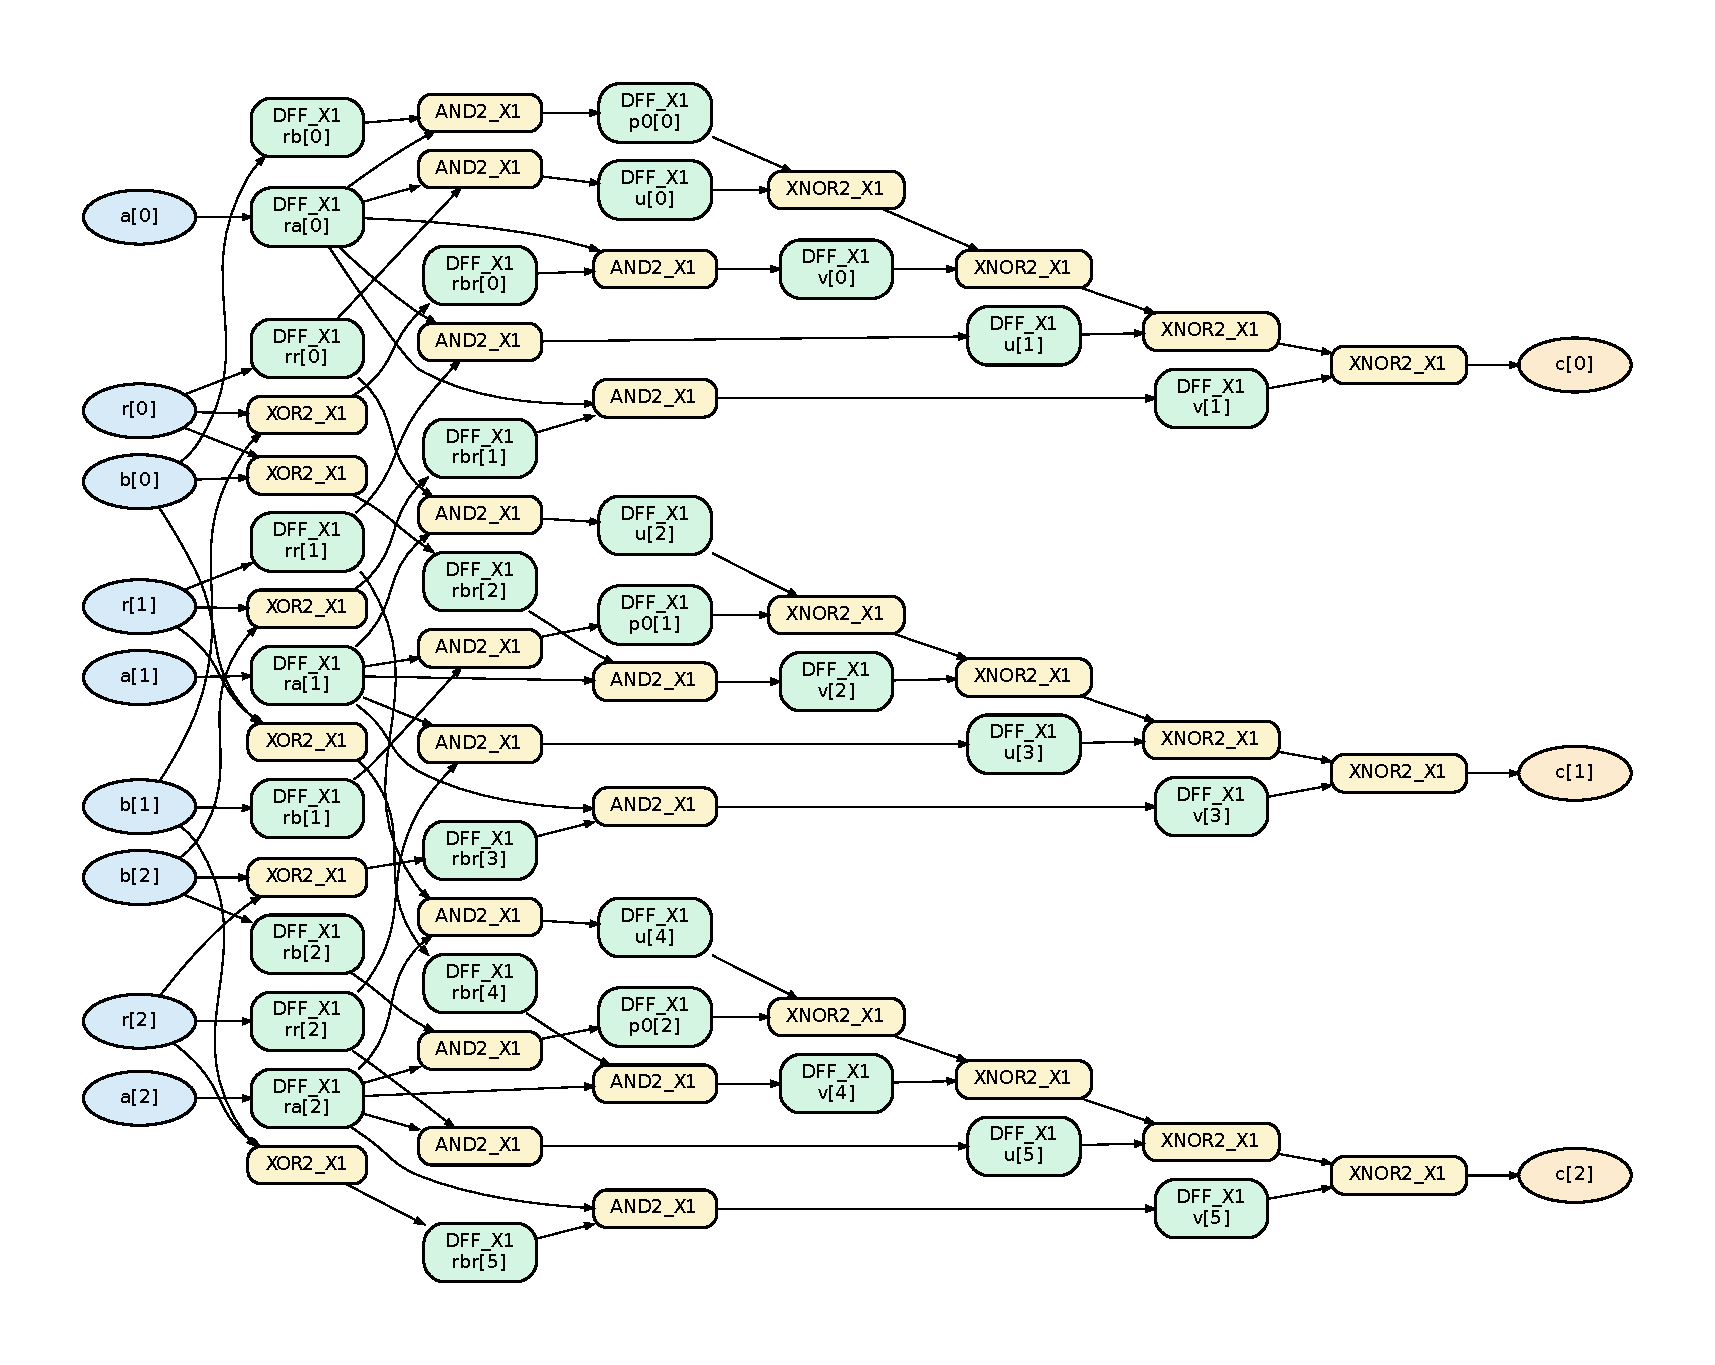
\includegraphics[width=0.92\textwidth]{figures/gates/hpc2_mapped.pdf}
\caption{The actual mapped HPC2 gadget (variant v0) from \file{competitors/runs/syn\_pams\_jqr\_p0/mapped.json}: every cell and every connection of module \sig{hpc2} after Yosys/ABC mapping to Nangate45, drawn automatically with Graphviz (\file{paper/scripts/generate\_figures.py}). Green = flip-flops, labelled with their RTL register names; yellow = combinational cells; ellipses = gadget ports. Clock connections are omitted.}\label{fig:hpc2-mapped}
\end{figure}

\subsection{Pipeline and critical paths}\label{app:critpath}
\paragraph{Stage structure.} \Cref{tab:v-stages} gives the stages. Every stage boundary is a register, and every combinational path runs between two registers of adjacent stages, or from a register to the outputs \sig{cdec}/\sig{dec}.

\paragraph{Synthesis timing.} In synthesis STA (no wires), the worst register group of \sig{pams\_jqr} is the public \sig{lowrq} ($1.033\ns$ including setup). Close behind are the partial products \sig{ml0} ($1.016\ns$) and \sig{mh0} ($0.994\ns$), and the public \sig{qcr} ($0.925\ns$). The later share-wise stages have slack: \sig{s0p} needs $0.784\ns$ and \sig{y0} $0.620\ns$. In the baseline every share-wise stage needs about $1.0\ns$.

\paragraph{Routed critical path at 1.2\ns{} (seed 1).} From \file{timing.rpt}, on RCX parasitics with a propagated clock:
\begin{itemize}
  \item \emph{Launch.} The path starts at flip-flop \sig{\_8799\_}, whose Q is \sig{x1r[5]}, bit 5 of share 1 at stage 2. The clock arrives after $0.179\ns$ of clock-tree latency, and clock-to-Q takes $0.168\ns$.
  \item \emph{Logic.} It passes 21 combinational cells:
    \begin{itemize}
      \item eight cells (\sig{XOR2}, \sig{NOR2}, \sig{OAI21}, \sig{AND2}, \sig{XNOR2}, \sig{XOR2}, \sig{XNOR2}, \sig{NOR2}) forming the carry-save part of the constant multiplication;
      \item twelve AOI/OAI-type cells (\sig{AOI21}, \sig{OAI221}, \sig{AOI221}, \sig{OAI21}, \sig{NAND2}, then alternating \sig{AOI21}/\sig{OAI21}), the carry propagation of the partial-product adder;
      \item a final \sig{XOR2\_X1} for the sum bit.
    \end{itemize}
  \item \emph{Capture.} It ends at the D pin of \sig{\_8676\_}, whose Q is \sig{ml1[23]}, bit 23 of the low partial product of share 1. The data arrives at $1.236\ns$. The required time is $1.343\ns$ ($1.2\ns$ + capture clock latency $0.180\ns$ $-$ setup $0.037\ns$), so the slack is $+0.107\ns$.
\end{itemize}
The baseline's path, \sig{x0r[9]}$\to$\sig{mh0[31]}, is the corresponding partial product of its 34-bit constant, with a $1.073\ns$ data path and slack $+0.089\ns$. Neither design's critical path involves a gadget or the masked kernel.

\subsection{Physical placement and routing}\label{app:physical}
\Cref{fig:layout} shows the routed layouts as rendered by OpenROAD's own GUI renderer (\texttt{save\_image}, run headless). Both images use the same resolution, $0.1\,\si{\micro\meter}$ per pixel, downsampled by 2 for the document, so their sizes compare directly:
\begin{itemize}
  \item \PAMS{}: die $188.7\,\si{\micro\meter}$ wide, $2075 \times 2075$ pixels at full resolution;
  \item baseline: die $209.0\,\si{\micro\meter}$, $2299 \times 2299$ pixels.
\end{itemize}
What the renders show:
\begin{itemize}
  \item the horizontal power-grid straps (pink) and vertical straps;
  \item signal wiring on metal 2 and metal 3 (red/green; most of the wire length);
  \item the I/O pins on the boundary;
  \item the standard cells underneath.
\end{itemize}
Functional regions cannot be read from such a render. \Cref{fig:placement} therefore colours the same cells by class using the DEF.

\begin{figure}[h]\centering
\begin{subfigure}[t]{0.47\textwidth}\centering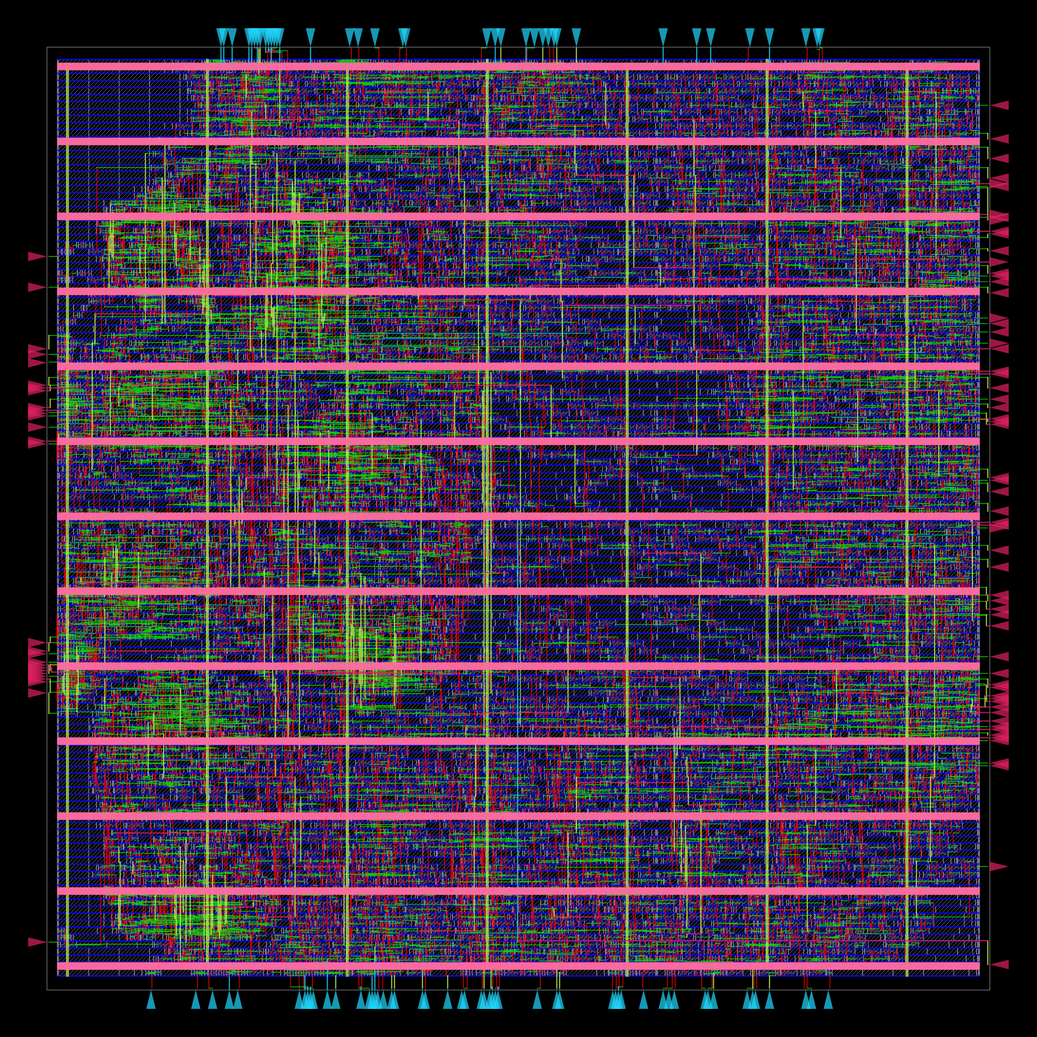
\includegraphics[width=0.903\linewidth]{figures/physical/layout_pams_jqr_half.png}\caption{\PAMS{} (\sig{pams\_jqr}), die $188.7^2\,\si{\micro\meter\squared}$}\end{subfigure}\hfill
\begin{subfigure}[t]{0.47\textwidth}\centering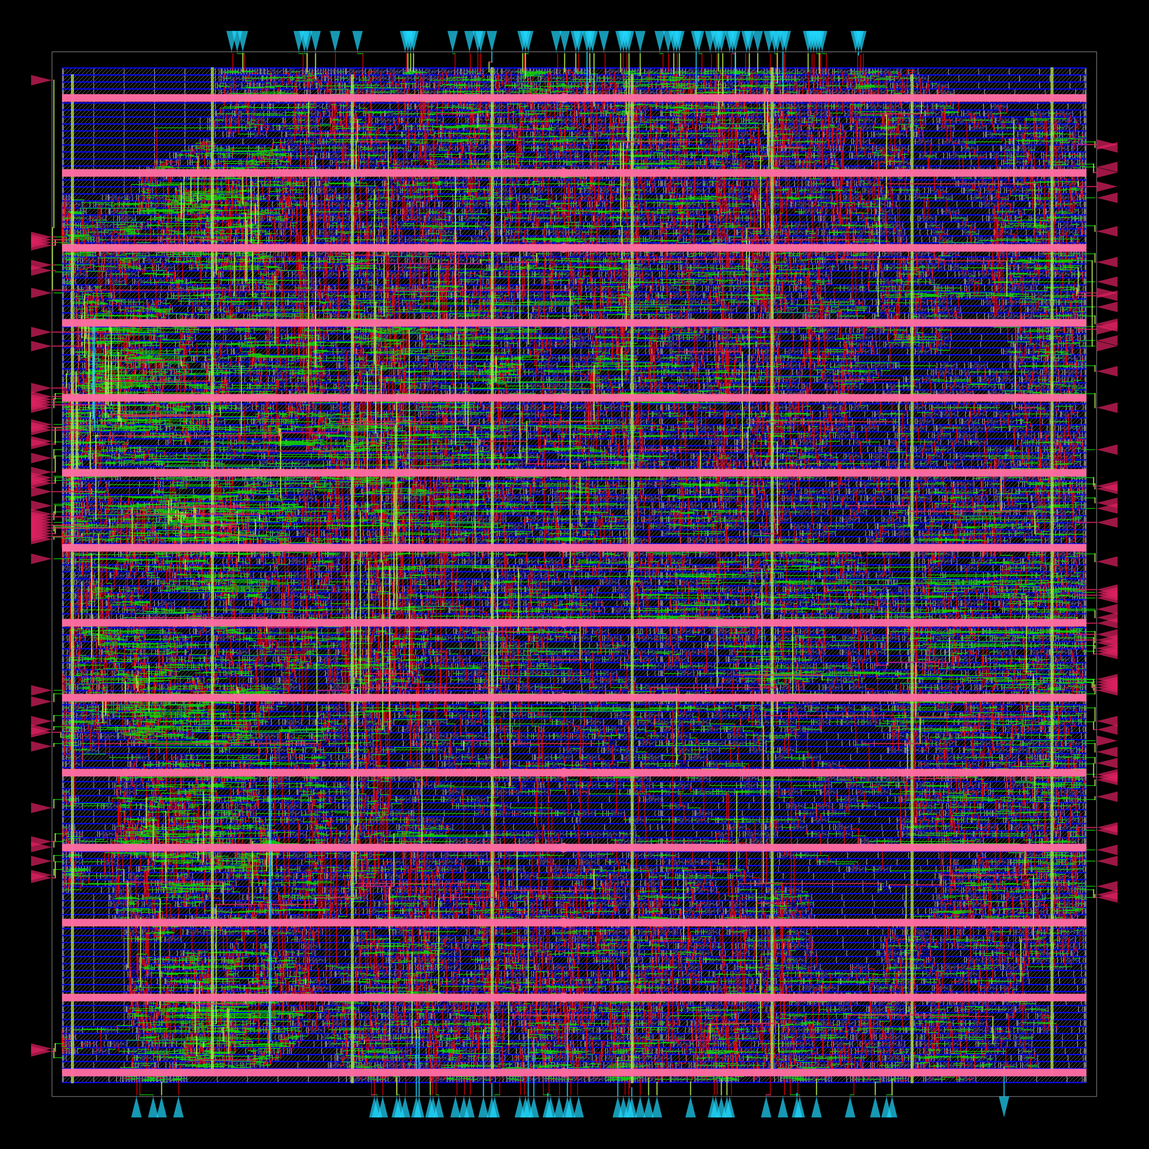
\includegraphics[width=\linewidth]{figures/physical/layout_base_jq_half.png}\caption{baseline (\sig{base\_jq}), die $209.0^2\,\si{\micro\meter\squared}$}\end{subfigure}
\caption{Routed layouts (target 1.2\ns, seed 1, utilization 50\,\%), rendered by OpenROAD (\texttt{save\_image}, $0.1\,\si{\micro\meter}$/pixel, downsampled $\times 2$) and shown at the same scale: the \PAMS{} image is $188.7/209.0 = 0.903$ of the baseline's width.}\label{fig:layout}
\end{figure}

\paragraph{Tool evidence for routability.} We do not infer congestion from appearance; \cref{tab:route-evidence} lists what the tools report.
\begin{itemize}
  \item \textbf{Detailed routing at 1.1\ns.} The router clears \PAMS{}'s initial violations in four iterations ($892 \to 98 \to 94 \to 0$). For baseline seed 2 it reaches 3 violations after three iterations and then oscillates between 2 and 11 violations for 50 further "stubborn tiles" iterations, ending at 3.
  \item \textbf{Hold buffering.} Hold fixing, which with I/O at the clock edge is the dominant source of buffers, inserts about 430--460 more buffers for the baseline. Its 3,210 clock sinks against 2,494 for \PAMS{} also make the clock tree larger.
\end{itemize}

\begin{table}[h]\centering\small
\caption{OpenROAD-reported routing quantities of representative runs.}\label{tab:route-evidence}
\begin{tabular}{@{}lrrrrr@{}}
\toprule
run & clock sinks & hold buffers & routed wire (\si{\micro\meter}) & DR iterations & final DRC \\
\midrule
\PAMS{} 1.2\ns{} s1 & 2,494 & 1,381 & 58,126 & 5 & 0 \\
baseline 1.2\ns{} s1 & 3,210 & 1,841 & 72,887 & 6 & 0 \\
\PAMS{} 1.1\ns{} s2 & 2,494 & 1,421 & 58,506 & 4 & 0 \\
baseline 1.1\ns{} s2 & 3,210 & 1,849 & 73,132 & 53 & 3 \\
baseline 1.1\ns{} s5 & 3,210 & 1,850 & 72,529 & 4 & 0 \\
\bottomrule
\end{tabular}
\end{table}

\subsection{Resource accounting}\label{app:resources}
\paragraph{How each count was obtained.}
\begin{itemize}
  \item \emph{Gadgets.} HPC2 instances in the RTL: 40 / 57. Synthesis and P\&R preserve them one-to-one (the G-check matches each routed gadget to the reference).
  \item \emph{Randomness.} The \sig{rnd} width: 3 bits per gadget, 120 / 171. The R-check verifies that each bit reaches exactly one gadget.
  \item \emph{Flip-flops.} \sig{DFF\_X1} count: 1,294 / 1,500 top-level plus 30 per gadget, i.e.\ 2,494 / 3,210 in total. These are also the clock sinks reported by CTS.
  \item \emph{Areas.} Liberty cell areas summed (synthesis) or OpenROAD \texttt{design\_area} (routed).
\end{itemize}

\paragraph{Functional decomposition.} \Cref{tab:resources-full} decomposes the synthesized area (\file{paper/scripts/resources.py}). Gadget cells are counted inside their hierarchy. Flip-flops are classified by the RTL name on their Q net. Every other combinational cell is assigned to the register group that its fan-out cone reaches first, and to "shared" if it reaches several. The decomposition sums exactly to the reported synthesis area, but the attribution of individual combinational cells is approximate where ABC shared logic between groups.

\begin{table}[h]\centering\small
\caption{Synthesized area by function, mapping 0 (cells, \si{\micro\meter\squared}).}\label{tab:resources-full}
\begin{tabular}{@{}lrrrr@{}}
\toprule
group & \multicolumn{2}{c}{\PAMS{}} & \multicolumn{2}{c}{baseline} \\
 & cells & area & cells & area \\
\midrule
HPC2 gadgets (63 cells / $180.35\um$ each) & 2,520 & 7,213.9 & 3,591 & 10,279.8 \\
FF: alignment (delay chains) & 782 & 3,536.2 & 876 & 3,961.3 \\
FF: partial products & 159 & 719.0 & 197 & 890.8 \\
FF: $x_r$, switched value, Yosys-named & 80 & 361.8 & 115 & 520.0 \\
FF: aligned operands $y_i$ & 42 & 189.9 & 72 & 325.6 \\
FF: public constants & 83 & 375.3 & 86 & 388.9 \\
FF: inputs, control, accumulator & 148 & 669.3 & 154 & 696.4 \\
logic $\to$ partial products & 1,972 & 2,274.0 & 1,968 & 2,406.0 \\
logic $\to$ switched value / Yosys-named & 305 & 335.7 & 444 & 626.7 \\
logic $\to$ aligned operands & 87 & 104.0 & 334 & 501.4 \\
logic $\to$ public constants & 783 & 961.3 & 70 & 75.0 \\
logic $\to$ gadget-input XOR network & 162 & 256.4 & 181 & 266.3 \\
logic $\to$ alignment, other, shared & 17 & 25.3 & 121 & 158.8 \\
\midrule
total & 7,140 & 17,022.1 & 8,209 & 21,097.0 \\
\bottomrule
\end{tabular}
\end{table}
